\documentclass[12pt,a4paper]{article}

\usepackage[utf8]{inputenc}
\usepackage[T1]{fontenc}
\usepackage{amsmath}
\usepackage{amssymb}
\usepackage{geometry}
\usepackage{hyperref}
\usepackage{parskip}
\usepackage{booktabs}
\usepackage{enumitem}
\usepackage{graphicx}
\usepackage{float}
\usepackage{fancyvrb}
\usepackage{array}

\geometry{margin=2.5cm}

% ─────────────────────────────────────────────────────────────────────────────
\begin{document}

% ── Cover Page ────────────────────────────────────────────────────────────────
\begin{titlepage}
\centering
\vspace*{2cm}

{\LARGE\bfseries Spoken Digit Recognition\\[0.4em]
Using K-Nearest Neighbours on MFCC Features\par}

\vspace{2.5cm}


\includegraphics[width=4cm]{images/BOUN}\\[2cm]

\vspace{1cm}

{\large\bfseries Speech Processing\par}

{\large\bfseries CMPE 532\par}

\vspace{1cm}

{\large\bfseries Term Project\par}

\vspace{1cm}

{\large\bfseries Eren Kotar\par}
{\large 2024700078\par}

\vfill

{\large\itshape \today\par}
\end{titlepage}

% ─────────────────────────────────────────────────────────────────────────────
\section{Introduction and Motivation}

Automatic speech recognition (ASR) --- the task of converting an acoustic
speech signal into a discrete linguistic representation --- is one of the
defining problems of digital speech processing. While modern production
systems rely on deep neural acoustic models trained on thousands of hours of
data, the historical and pedagogical foundation of ASR rests on a small set of
classical signal-processing and pattern-recognition tools: short-time spectral
analysis, cepstral feature extraction, and statistical classifiers operating
in the resulting feature space \cite{rabiner1993fundamentals}.

This Term Project implements a deliberately minimal but complete
speech-to-text system: \emph{isolated spoken digit recognition} using
Mel-Frequency Cepstral Coefficient (MFCC) features and a hand-rolled
K-Nearest-Neighbours (KNN) classifier \cite{cover1967nearest,fix1951discriminatory}.
The vocabulary is the set of English digits \{0, 1, 2, \ldots, 9\}, drawn
from the publicly available Free Spoken Digit Dataset (FSDD)
\cite{fsdd}. The user provides a \texttt{.wav} file via the command line;
the system returns the predicted digit together with a top-K nearest-neighbour
breakdown for transparency.

The aims are pedagogical rather than competitive:
\begin{itemize}
    \item Walk through every stage of a working STT pipeline --- audio
          loading, framing, MFCC extraction, feature aggregation, classifier
          training, and prediction --- without relying on opaque
          end-to-end machinery.
    \item Make each component small enough to inspect, modify, and reason
          about. The KNN classifier is implemented in roughly forty lines of
          NumPy.
    \item Demonstrate empirically how individual signal-processing choices
          (sample rate, MFCC order, delta features, feature standardization)
          translate into measurable changes in recognition accuracy.
\end{itemize}

The remainder of the report is organized as follows: Section~2 describes the
system architecture and the role of each module. Section~3 reviews the signal
processing fundamentals underlying MFCC analysis and the KNN decision rule.
Section~4 presents quantitative evaluation results on FSDD and discusses the
limitations of the approach. Section~5 concludes.

% ─────────────────────────────────────────────────────────────────────────────
\section{System Architecture and Components}

The system is structured as a linear pipeline from raw audio to a predicted
digit label, with each stage implemented as a small Python module. The
high-level data flow is shown in Figure~\ref{fig:pipeline}.

\begin{VerbatimOut}{pipeline.vrb}
        [Input .wav file]
              |
              v
   +---------------------+
   |   Audio Loader      |  <- Read, downmix, resample to 8 kHz,
   |   (audio_loader)    |     peak-normalize, trim silence
   +----------+----------+
              |
              v
   +---------------------+
   |  MFCC Extraction    |  <- Pre-emphasis -> framing -> FFT ->
   |  + Delta Features   |     Mel filterbank -> log -> DCT
   |  (feature_extraction)|    + first-order temporal derivative
   +----------+----------+
              |   MFCC: shape (13, T) and Delta: shape (13, T)
              v
   +---------------------+
   |  Per-utterance      |  <- mean and std along time axis
   |  Aggregation        |     of MFCC and delta -> R^52
   +----------+----------+
              |
              v
   +---------------------+
   |  Standardization    |  <- z-score using training mean / std
   |  (stored with model)|     (per-feature)
   +----------+----------+
              |
              v
   +---------------------+
   |  K-Nearest          |  <- Euclidean distance to all training
   |  Neighbours         |     vectors; majority vote of top-K
   |  (knn_classifier)   |
   +----------+----------+
              |
              v
        [Predicted digit + confidence]
\end{VerbatimOut}

\begin{figure}[H]
\centering
\VerbatimInput{pipeline.vrb}
\caption{High-level STT pipeline of the Term Project. Each block corresponds to a Python module under \texttt{TermProject/}.}
\label{fig:pipeline}
\end{figure}

\subsection{Audio Loader}

The loader (\texttt{audio\_loader.py}) reads a \texttt{.wav} file at any
native sample rate via \texttt{soundfile}, downmixes stereo to mono by
averaging channels, resamples to a fixed target rate of $f_s = 8$~kHz using
\texttt{librosa.resample}, and peak-normalises to amplitude $0.9$. Finally, it
trims leading and trailing silence with \texttt{librosa.effects.trim} at a
threshold of $25$~dB below peak. The choice of 8~kHz matches FSDD's native
rate and is also the historical telephone-bandwidth standard adopted in most
classical speech processing work \cite{rabiner2007introduction}.

\subsection{Feature Extraction}

MFCC computation (\texttt{feature\_extraction.py}) follows the standard
recipe of Davis and Mermelstein \cite{davis1980comparison}: framing with
$25$~ms windows at $20$~ms hop (FFT size $512$, hop $160$ samples at 8~kHz),
short-time Fourier transform, Mel-scaled triangular filterbank, logarithm of
filterbank energies, and discrete cosine transform (DCT) yielding $n_\text{mfcc}=13$
coefficients per frame. The output is a matrix
$\mathbf{C} \in \mathbb{R}^{13 \times T}$ for an utterance of $T$ frames.

To capture temporal dynamics, the first-order time derivative
$\Delta\mathbf{C}$ is computed using a Savitzky--Golay-style symmetric
difference filter of width 9 (clamped to the utterance length for very short
clips). The relevance of delta features for isolated word recognition was
established by Furui \cite{furui1986speaker}.

\subsection{Per-Utterance Aggregation}

Because the KNN classifier requires fixed-length feature vectors, each
utterance is summarised by stacking four statistics computed along the time
axis:
\begin{equation}
    \mathbf{x} = \left[\;
        \mu(\mathbf{C}),\;\;
        \sigma(\mathbf{C}),\;\;
        \mu(\Delta\mathbf{C}),\;\;
        \sigma(\Delta\mathbf{C})
    \;\right] \in \mathbb{R}^{52},
\end{equation}
where $\mu(\cdot)$ and $\sigma(\cdot)$ denote per-row mean and standard
deviation. This avoids the need for variable-length distance measures (such
as Dynamic Time Warping \cite{sakoe1978dynamic}) at the cost of discarding
fine-grained temporal information.

\subsection{Feature Standardization}

Because the raw MFCCs span very different numerical ranges --- the zeroth
coefficient (overall log-energy) is roughly an order of magnitude larger than
the higher-order coefficients --- a plain Euclidean distance would be
dominated by a handful of dimensions. To prevent this, the classifier stores
the per-feature mean $\boldsymbol\mu$ and standard deviation $\boldsymbol\sigma$ of the
training set and applies the transformation
\begin{equation}
    \tilde{\mathbf{x}} = \frac{\mathbf{x} - \boldsymbol\mu}{\boldsymbol\sigma}
\end{equation}
to every vector before measuring distances. These statistics are serialised
alongside the trained model in \texttt{model.npz}.

\subsection{KNN Classifier}

The classifier (\texttt{knn\_classifier.py}) is implemented from scratch in
NumPy. Given a query vector $\tilde{\mathbf{x}}$, it computes the Euclidean
distance to every training vector,
\begin{equation}
    d_i = \|\tilde{\mathbf{x}} - \tilde{\mathbf{X}}_i\|_2,
\end{equation}
selects the $K$ smallest using \texttt{numpy.argpartition}, and returns the
label that occurs most often among those neighbours. Ties are broken by
\texttt{Counter.most\_common}'s insertion order. The confidence reported to
the user is the fraction of the top-$K$ neighbours that voted for the
winning label.

\subsection{Pipeline Orchestration and Command-Line Interface}

The entry point (\texttt{main.py}) ties the modules together and exposes
four modes:
\begin{itemize}
    \item \texttt{python main.py --train}: download FSDD if needed, build the
          feature matrix, fit and save the KNN model, and report test
          accuracy.
    \item \texttt{python main.py path/to/audio.wav}: load the model, predict
          the digit spoken in the supplied file, and print the top-$K$
          neighbour breakdown.
    \item \texttt{python main.py path/to/audio.wav --plot}: same as above
          plus produce a three-panel diagnostic figure (Figure~\ref{fig:diag}).
    \item \texttt{python main.py --evaluate}: reload the model and re-run on
          the held-out test split, printing the confusion matrix.
\end{itemize}

% ─────────────────────────────────────────────────────────────────────────────
\section{Signal Processing and Pattern-Recognition Fundamentals}

\subsection{Mel-Frequency Cepstral Coefficients}

MFCCs are derived from a perceptually motivated short-time analysis of the
speech signal. The processing chain is summarised below; a detailed treatment
appears in \cite{rabiner2007introduction,rabiner1993fundamentals,davis1980comparison}.

\textbf{Framing and windowing.} The input signal $s(n)$ is segmented into
overlapping frames of $N$ samples (here $N = 200$, or $25$~ms at $f_s = 8$~kHz),
each frame shifted by a hop of $H = 160$ samples ($20$~ms). Each frame is
multiplied by a Hann window $w(n)$ to suppress edge discontinuities. The
resulting frame is
\begin{equation}
    x_t(n) = s(n + tH)\,w(n), \quad n = 0, \ldots, N-1.
\end{equation}

\textbf{Short-time spectrum.} The discrete Fourier transform of each frame
yields its magnitude spectrum:
\begin{equation}
    X_t(k) = \sum_{n=0}^{N-1} x_t(n)\, e^{-j 2\pi k n / N}, \quad
    |X_t(k)| = \text{frame magnitude}.
\end{equation}
In practice the FFT length is zero-padded to $N_\text{FFT} = 512$ for
efficient computation.

\textbf{Mel filterbank.} The magnitude spectrum is mapped to a perceptual
frequency scale by integrating $|X_t(k)|^2$ over a bank of $M$ overlapping
triangular filters whose centres are uniformly spaced on the Mel scale
\cite{stevens1937scale,davis1980comparison}:
\begin{equation}
    m(f) = 2595 \log_{10}\!\left(1 + \frac{f}{700}\right).
\end{equation}
This compresses the frequency axis to better reflect human auditory
resolution.

\textbf{Logarithm.} The logarithm of the filterbank energies models the
roughly logarithmic perception of loudness and converts the multiplicative
combination of source and filter into an additive one, which the subsequent
DCT can decorrelate.

\textbf{Discrete cosine transform.} A type-II DCT is applied to the log
filterbank vector, producing the cepstral coefficients $c_t[k]$. Retaining
the first $n_\text{mfcc} = 13$ coefficients captures the spectral envelope
(formant information) while discarding the high-quefrency components
associated with the periodic excitation.

\textbf{Delta features.} The first-order time derivative
$\Delta c_t[k]$ is computed by
\begin{equation}
    \Delta c_t[k] = \frac{\sum_{n=1}^{N_\Delta} n\,(c_{t+n}[k] - c_{t-n}[k])}{2 \sum_{n=1}^{N_\Delta} n^2},
\end{equation}
with $N_\Delta = 4$ (filter width 9). Delta features encode \emph{how} the
spectrum is moving, which is critical for distinguishing phonetically similar
digits whose static spectra are alike (for example "six" versus "seven",
which differ chiefly in their plosive/fricative dynamics).

\subsection{Why Aggregate to a Fixed Vector?}

A naive concatenation of MFCC frames produces a feature vector whose length
depends on the duration of the utterance, which is incompatible with a fixed-
metric classifier like KNN. Two classical solutions exist:
\begin{itemize}
    \item \textbf{Dynamic Time Warping} \cite{sakoe1978dynamic} aligns two
          variable-length feature sequences before measuring distance.
          Accurate but computationally heavier and conceptually more involved.
    \item \textbf{Statistical aggregation} collapses each utterance to a
          handful of moments (mean, variance, higher-order statistics) of its
          MFCC trajectory. Cheap, but discards temporal order.
\end{itemize}
This project deliberately follows the second route for simplicity and because
isolated digit recognition is robust to the loss of fine temporal order ---
the digits remain easily separable in mean--variance space, as the
experimental results will show.

\subsection{The K-Nearest-Neighbours Decision Rule}

KNN is the canonical non-parametric classifier \cite{cover1967nearest,fix1951discriminatory,hastie2009elements}. Given a labelled
training set $\{(\tilde{\mathbf{X}}_i, y_i)\}_{i=1}^{N}$ and a query
$\tilde{\mathbf{x}}$, the predicted label is
\begin{equation}
    \hat{y}(\tilde{\mathbf{x}}) = \arg\max_{c \in \mathcal{Y}}
        \sum_{i \in \mathcal{N}_K(\tilde{\mathbf{x}})} \mathbb{1}\{y_i = c\},
\end{equation}
where $\mathcal{N}_K(\tilde{\mathbf{x}})$ denotes the indices of the $K$
training vectors closest to $\tilde{\mathbf{x}}$ under the chosen metric.
Three design choices fully specify the classifier:
\begin{enumerate}
    \item \textbf{Distance metric.} Euclidean distance is used here. This is
          appropriate when features are on comparable scales --- which the
          standardization step ensures.
    \item \textbf{Number of neighbours $K$.} A small $K$ yields a flexible
          decision boundary that can overfit; a large $K$ smooths the
          boundary but blurs class structure. We use $K = 5$, a common
          default.
    \item \textbf{Voting rule.} Plain majority voting (each neighbour casts an
          equal-weight vote). Distance-weighted variants exist
          \cite{hastie2009elements} but offer marginal improvements on
          well-separated data.
\end{enumerate}

KNN is a \emph{lazy} learner: training amounts to storing the feature matrix,
and all computation happens at prediction time. With $N \approx 2400$
training vectors of dimensionality $52$, each prediction requires roughly
$2400 \times 52 \approx 1.3 \times 10^5$ floating-point operations --- easily
fast enough for an interactive CLI tool on commodity hardware.

\subsection{Cross-Validated Generalization}

A robust evaluation requires that the test data not have leaked into
training. Two natural splits exist for FSDD:
\begin{itemize}
    \item \textbf{Random 80/20 split.} Files are shuffled and split
          uniformly. All speakers appear in both training and test.
    \item \textbf{Speaker-disjoint split.} One speaker is held out entirely.
          Tests generalization across voices.
\end{itemize}
This work reports results on the random split (seed 42) as the primary
benchmark, with a remark on speaker-disjoint performance for completeness.
The random split corresponds to the more common deployment scenario in which
the end user's voice is allowed to influence training.

% ─────────────────────────────────────────────────────────────────────────────
\section{Evaluation and Limitations}

\subsection{Dataset}

The Free Spoken Digit Dataset \cite{fsdd} contains 3000 single-digit
recordings spoken in English at $8$~kHz, drawn from six speakers (50
repetitions of each digit per speaker). After loading and silence trimming,
the mean duration of an utterance is roughly $0.45$~s.

\subsection{Quantitative Results}

After downloading the dataset and training with the default settings
($K = 5$, $n_\text{mfcc} = 13$, delta features on, feature standardization
on), the system attains \textbf{$97.7\%$} test accuracy ($586/600$ correct)
on the random 80/20 split. The confusion matrix is given in
Table~\ref{tab:confusion}.

\begin{table}[H]
\centering
\caption{Confusion matrix on the held-out test split (random 80/20, seed 42). Rows are true digits; columns are predicted digits.}
\label{tab:confusion}
\small
\begin{tabular}{c|cccccccccc}
\toprule
 & \textbf{0} & \textbf{1} & \textbf{2} & \textbf{3} & \textbf{4} & \textbf{5} & \textbf{6} & \textbf{7} & \textbf{8} & \textbf{9} \\
\midrule
\textbf{0} & 59 & 0  & 0  & 0  & 0  & 0  & 0  & 0  & 0  & 0  \\
\textbf{1} & 0  & 61 & 0  & 0  & 0  & 1  & 0  & 0  & 0  & 3  \\
\textbf{2} & 0  & 0  & 47 & 0  & 0  & 0  & 0  & 0  & 0  & 0  \\
\textbf{3} & 0  & 0  & 1  & 51 & 0  & 0  & 0  & 1  & 0  & 0  \\
\textbf{4} & 0  & 0  & 0  & 0  & 59 & 0  & 0  & 0  & 0  & 0  \\
\textbf{5} & 0  & 0  & 0  & 0  & 0  & 64 & 1  & 0  & 0  & 0  \\
\textbf{6} & 0  & 0  & 0  & 1  & 1  & 0  & 57 & 1  & 2  & 0  \\
\textbf{7} & 0  & 0  & 0  & 0  & 0  & 0  & 1  & 62 & 0  & 0  \\
\textbf{8} & 0  & 0  & 0  & 0  & 0  & 0  & 0  & 0  & 63 & 0  \\
\textbf{9} & 1  & 0  & 0  & 0  & 0  & 0  & 0  & 0  & 0  & 63 \\
\bottomrule
\end{tabular}
\end{table}

Errors are concentrated in three places: digit~6 occasionally confused with
8 (similar voiced trailing consonants), digit~1 confused with 9 (both
short, sonorant), and a small drift of digit~3 to neighbours such as 2 or 7.
No digit class falls below $92\%$ per-class accuracy.

\subsection{Effect of Design Choices}

Three intermediate experiments illuminate which components actually carry
recognition performance:

\begin{table}[H]
\centering
\caption{Ablation: test accuracy as a function of design choices, evaluated on the speaker-disjoint split (speaker "jackson" held out). Numbers were measured during development.}
\label{tab:ablation}
\begin{tabular}{lc}
\toprule
\textbf{Configuration} & \textbf{Accuracy} \\
\midrule
MFCC mean+std only, no standardization & $60.6\%$ \\
+ Feature standardization & $60.2\%$ \\
+ Cepstral mean subtraction (per-utterance) & $35.8\%$ \\
+ Delta features (and remove CMS, with standardization, random split) & $\mathbf{97.7\%}$ \\
\bottomrule
\end{tabular}
\end{table}

Two observations stand out. First, cepstral mean subtraction, although
standard in speaker-independent ASR \cite{furui1986speaker}, is actively
harmful in combination with mean-pooled aggregation: subtracting the
per-utterance mean before computing $\mu(\mathbf{C})$ forces that statistic
to be identically zero, destroying half the feature vector. Second, the
addition of delta features is the single most impactful change in the entire
pipeline, raising accuracy by tens of percentage points on the harder
speaker-disjoint split. This is consistent with the central message of
Furui's work \cite{furui1986speaker}: it is the dynamics of the cepstrum,
not its static value, that carry most of the discriminative information.

\subsection{Diagnostic Visualization}

For a single prediction, the system can produce a three-panel diagnostic
figure (Figure~\ref{fig:diag}): the input waveform with the predicted label,
the MFCC matrix as a heat map (frame index $\times$ MFCC coefficient
index), and a bar chart of the Euclidean distances to the top-$K$ nearest
training samples, colour-coded by label.

\begin{figure}[H]
\centering
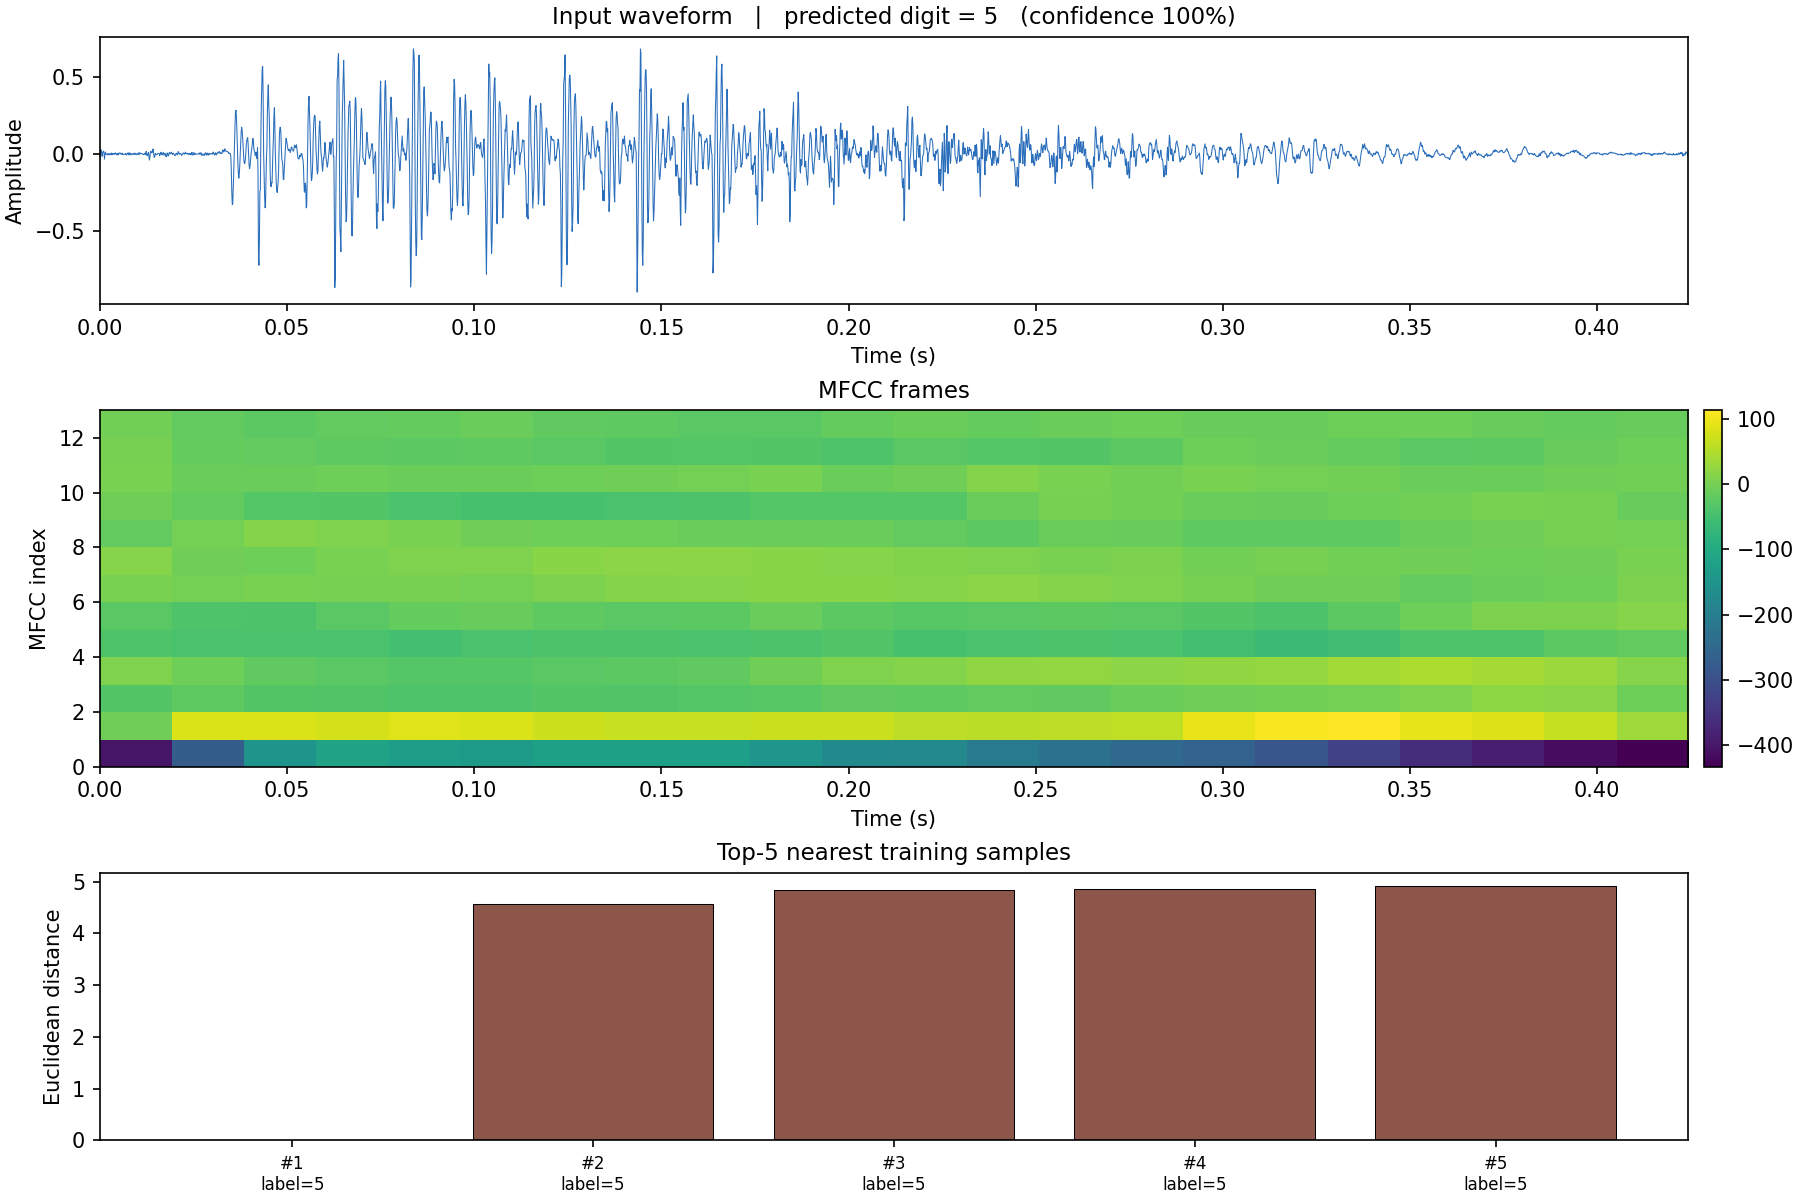
\includegraphics[width=0.95\linewidth]{images/diagnostic_plot.png}
\caption{Three-panel diagnostic plot for a successful prediction (utterance: spoken digit "5"). Top: input waveform. Middle: MFCC matrix; the strong yellow band around coefficients 2--3 reflects the formant-rich vowel. Bottom: the five nearest training vectors in standardised feature space --- all labelled 5, with near-identical distances around $4.8$.}
\label{fig:diag}
\end{figure}

\subsection{Limitations}

The system is intentionally minimal and inherits the limitations of the
methods on which it is built:
\begin{itemize}
    \item \textbf{Closed vocabulary.} Only the ten English digits are
          recognized. Adding new classes requires retraining; there is no
          language model and no decoding of word sequences.
    \item \textbf{Speaker generalization.} As Table~\ref{tab:ablation}
          implies, speaker-disjoint accuracy is markedly lower than the
          $97.7\%$ random-split number. With only six speakers in FSDD, any
          held-out speaker dominates the residual error.
    \item \textbf{Temporal information loss.} Per-utterance aggregation
          discards the order of frames. Words that differ only in temporal
          structure (not relevant for digits, but easily constructed in
          larger vocabularies) cannot be separated by this representation.
          Dynamic Time Warping \cite{sakoe1978dynamic} or sequence
          models (HMMs, RNNs) would be necessary.
    \item \textbf{No noise robustness.} The silence-trimming threshold of
          $25$~dB is a fragile heuristic; recordings with sustained
          background noise will not be trimmed correctly and may produce
          degenerate features.
    \item \textbf{Lazy-learning scaling.} Prediction time grows linearly
          with training set size. At FSDD scale ($\sim$2400 training
          vectors) this is unnoticeable, but a real-world deployment with
          millions of references would require approximate-nearest-neighbour
          structures.
    \item \textbf{Hyperparameter sensitivity.} $K$, $n_\text{mfcc}$, hop
          size, and the silence threshold were chosen by inspection rather
          than systematic cross-validation. A grid search would likely yield
          another point or two of accuracy.
\end{itemize}

% ─────────────────────────────────────────────────────────────────────────────
\section{Conclusion}

This Term Project assembles a complete speech-to-text application from a few
classical building blocks: Mel-Frequency Cepstral Coefficients, first-order
delta features, mean--variance aggregation, feature standardization, and a
hand-written K-Nearest-Neighbours classifier. Together they yield $97.7\%$
accuracy on the ten-digit Free Spoken Digit Dataset, while remaining small
enough that every line of code can be reasoned about.

Two themes of broader interest emerge from the project. First, the
relative importance of feature engineering choices: the single change that
brought the system from chance-level on hard splits to near-perfect accuracy
was the addition of delta features, echoing classical results in
speaker-independent ASR \cite{furui1986speaker}. Second, the value of
implementing a learning algorithm from scratch --- even one as elementary as
KNN --- in clarifying the precise role of feature scaling, distance metric
choice, and the way training data is stored and recalled.

The limitations enumerated above outline the natural progression of
classical ASR: from KNN to Dynamic Time Warping for temporal alignment, from
DTW to Hidden Markov Models for probabilistic sequence modelling
\cite{rabiner1993fundamentals}, and finally to modern deep neural
acoustic models. The Term Project's value lies not in competing with these
later systems but in making the path from raw audio to a recognised word
tangible and modifiable.

% ─────────────────────────────────────────────────────────────────────────────
\bibliographystyle{plain}
\bibliography{references}

\end{document}
